\section{Methodology}
I first fine-tune two pre-trained models,  a stable diffusion model with the v1.5 checkpoint weights \cite{rombach2022high} and ControlNet \cite{zhang2023adding} on the Transient Attribute Dataset \cite{laffont2014transient}. 

\subsection{Transient Attribute Dataset} 

The dataset consists of  8571 images captured from 101 webcams, all annotated with 40 attribute labels. In order to capture static viewpoints over long periods, the authors choose a group of outdoor webcams from the following existing sources: the Archive of Many Outdoor Scenes \cite{jacobs2007consistent} and the Webcam Clip Art Dataset \cite{lalonde2009webcam}. The dataset includes images of scenes with large variations, ranging from  mountainous views to urban areas with resolutions varying between $640 \times 360$ and $4000 \times 3000$. Images captured from the same webcam are also manually aligned to a reference frame with a warping method.
\paragraph{Attribute labels.} are selected with crowdsourcing from an initial list of 92 scene attributes. In the a crowdsourced experiment on Amazon Mechanical Turk, the authors observe that some properties rarely occur or do not vary across scenes, while weather-, lighting-, or emotion-related properties can change dramatically across the images of the same scene. This leads  to a reduced number of attributes (40) in five categories (lighting, weather, seasons, subjective impressions, additional attributes).

The attributes are as follows: \textit{dirty, daylight, night, sunrise sunset, dawn dusk, sunny, clouds, fog, storm,snow
, warm, cold, busy, beautiful, flowers, spring, summer, autumn, winter, glowing, colourful, dull, rugged, midday, dark
, bright, dry, moist, windy, rain, ice, cluttered, soothing, stressful, exciting, sentimental, mysterious, boring, gloomy, lush}.

Each image is later annotated with the corresponding attributes by the workers on Amazon Mechanical Turk. As attributes lie on a continuous spectrum, the workers are asked to answer "totally / a little / not at all" to the question "how much each image exhibits this attribute". These answers are later assigned to label values 1 / 0.5 / 0, and aggregated scores ranging from 0 (attribute not present) to 1 (attribute present) are estimated with a two-stage estimator. More details about the workers' performance and the estimation approach can be found in Section 3.2 in the main paper \cite{laffont2014transient}.

\subsection{Transient Attribute Transfer}
\paragraph{Fine-tuning.} Following their convention for the attributes list, I select the annotations with scores$ > 0.8$ to generate the associated text prompts of the images. In cases where images have multiple annotations with high scores, I merge them with a comma split. For example, if an image has high scores for both the 'sunny' and 'daylight' annotations, then the text prompt is 'daylight, sunny'. I fine-tune the models with  8571 images conditioned with the text prompts (attribute labels). For the fine-tuning of the models, I reform the dataset following the instructions given in the models' official GitHub repository. I only fine-tune the U-net parameters, freezing the parameters of all other components (encoders and decoders). 
\TODO{GPU info and how long you trained}

\TODO{explain DDIM and DDPM in background}
\paragraph{DDIM inversion.} To guide the input image with a latent diffusion model, I utilise \gls{DDIM} inversion, which inverts the DDIM sampling process by adding noise to the input image. Here, the idea is to start the sampling process from the noisy input image instead of a pure random noise. Figure \ref{fig:ddim-inversion} shows that the input image gradually turns into a random noise with the increasing number of time steps. Instead of using the random noise generated at the last step, if I start from, let's say, somewhere middle, then I can preserve the main structures of the input image (third subfigure in Figure \ref{fig:ddim-inversion}). Later, while sampling an output image with this intermediate latent, the priors embedded in the pre-trained model can steer the noisy input image towards a target image with the text guidance.

\begin{figure}[ht]
  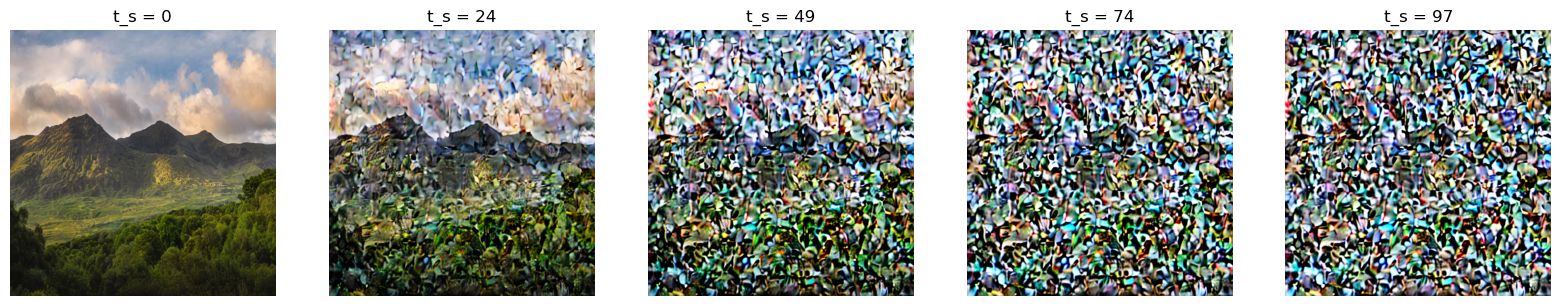
\includegraphics[width=\textwidth]{Chapters/zero-shot-tat-figs/DDIM_forward.png}
  \caption{In the forward process of a diffusion model, an input image gradually turns into a random noise by adding small amounts of Gaussian noise at each time step. Here, the total number of time steps is 100. In DDIM inversion, the sampling process replaces the random noise with an intermediate time step, such as $t_s = 49$, for its starting point.}
  \label{fig:ddim-inversion}
\end{figure}

Note that I use a latent diffusion model; hence, the noising process indeed occurs in the latent space. Here, I decode the noised latents with the VAE decoder of the model for visualisation. 

\paragraph{DDIM sampling.}
At a given time step $t$, the noisy image $\bm{x}_t$ is the original image ($\bm{x}_0$) mixed with some noise ($\epsilon$), mathematically defined as follows (from the DDIM paper \cite{song2020denoising}):

\begin{equation}
\bm{x}_t = \sqrt{\alpha_t}\bm{x}_0 + \sqrt{1 - \alpha_t}\epsilon
\end{equation}
where $\epsilon$ is some gaussian noise with unit variance, $\alpha_t$ is the noise scheduler. 

Sampling starts with pure noise at time step $T$ and gradually approaches $t = 0$. The next $\bm{x}_{t-1}$ in the sampling trajectory is calculated by predicting the noise $\epsilon\theta(\bm{x}_t)$ with the learned model, which is used to predict $\bm{x}_0$. The noise prediction is also incorporated into the "step" towards $\bm{x}_t$. The noise can also by added with a scale $\sigma_t$:

\begin{equation}
\bm{x}_{t -1} = \sqrt{\alpha_{t - 1}}\biggl(\frac{\bm{x}_t - \sqrt{1 - \alpha_t}\epsilon_{\theta}^{(t)}(\bm{x}_t)}{\sqrt{\alpha_t}}\biggl) + \sqrt{1 - \alpha_{t - 1} - \sigma_t^2} \, . \, \epsilon_{\theta}^{(t)}(\bm{x}_t) + \sigma_t \, \epsilon_t
\label{eq:ddim-sample}
\end{equation}
Here, the first term inside the parenthesis is the "predicted $\bm{x}_0$" multiplied with the noise scheduler, and the second term is the "direction pointing to $\bm{x}_t$". In my experiments, I do not add any additional noise term ($\sigma_t = 0$) to keep the sampling process fully deterministic. That is, samples follow a fixed procedure from $\bm{x}_T$ to $\bm{x}_0$.

Another important term to mention before discussing the experiment results is the \textbf{guidance scale}. A pre-trained U-net model predicts the noise $\epsilon_t$ at each time step. In the text-conditional case, the noise prediction includes one term for the unconditional prediction, and one for the text-conditioned prediction. The output noise prediction becomes the weighted average of these two with a guidance scale $\sigma_s$:
$$\epsilon_{pred} = \epsilon_{uncond} + \sigma_s * (\epsilon_{text} - \epsilon_{uncond} )$$.
\TODO{Double check this part from the main paper -- what is the difference between classifier-free vs }

%here: \href{https://github.com/lllyasviel/ControlNet}{ControlNet}, \href{https://github.com/timothybrooks/instruct-pix2pix}{Stable Diffusion v1.5}. 